
\documentclass[12pt,a4paper]{article}
\usepackage[utf8]{inputenc}
\usepackage[OT1]{fontenc}
\usepackage[russian]{babel}
\usepackage{amsmath}
\usepackage{amsfonts}
\usepackage{amssymb}
\usepackage{hyperref}
\hypersetup{linktoc=all}
\usepackage{indentfirst}
\usepackage[left=2cm,right=2cm,top=2cm,bottom=2cm]{geometry}
\usepackage{graphicx}
\usepackage{float}
\author{Борисенков Никита Николаевич}
\title{Отчёт}

\newcommand{\xo}{\mathring{x}}
\newcommand{\xx}{x\overline{x}}
\newcommand{\pd}[2]{\dfrac{\partial #1}{\partial #2}}
\DeclareMathOperator*{\mmax}{max}

\begin{document}
\maketitle
\tableofcontents
\newpage
\section{Постановка задачи}

Решается задача моделирования теплопроводного вязкого баротропного газа.

$$
\begin{array}{rcl}
    \pd{\rho}{t} + \pd{\rho u}{x} & = & 0\\
    \pd{\rho u}{t} + \pd{\rho u^2}{x} + \pd{p}{x} & = & \mu\pd{^2 u}{x^2} + \rho f
\end{array}
$$

\section{Алгоритм}

Используется последовательная схема с центральными разностями ($u, \rho$)

Уравнения, задающие схему выглядят следующим образом:
$$
\begin{array}{lc}
    V_t + \frac13 \left( V\hat{V}_{\xo} + ( V\hat{V} )_{\xo} \right) + \dfrac{p\left(H\right)_{\xo}}{H} = \tilde{\mu}\hat{V}_{\xx} - \left( \tilde{\mu} - \dfrac{\mu}{H} \right)V_{\xx} + f, & x \in \omega_h, \\

    H_t + 0,\!5 \left(  \hat{V}\hat{H}_{\xo} + (\hat{V}\hat{H})_{\xo} + H\hat{V}_{\xo}\right) = f_0, & x \in \omega_h, \\

    H_{t,0} + 0,\!5\left((\hat{V}\hat{H})_{x,0} + H_0\hat{V}_{x,0}\right) - & \\
    - 0,\!5h\left(\left(HV\right)_{\xx,1} - 0,\!5\left(HV\right)_{\xx,2} + H_0\left(V_{\xx,1} - 0,\!5V_{\xx,2}\right)\right) = f_0, & \\

    H_{t,M} + 0,\!5\left((\hat{V}\hat{H})_{\overline{x},M} + H_0\hat{V}_{\overline{x},M}\right) + & \\
    + 0,\!5h\left(\left(HV\right)_{\xx,M-1} - 0,\!5\left(HV\right)_{\xx,M-2} + H_0\left(V_{\xx,M-1} - 0,\!5V_{\xx,M-2}\right)\right) = f_0, & 
\end{array}
$$
где $\tilde{\mu} = \displaystyle\max_{m} \dfrac{\mu}{H}$.

По этим уравнениям сначала строится СЛУ на значения $V$ на следующеми слое, которое решается методом прогонки, а с использованием полученных значений $\hat{V}$ строится и решается СЛУ на $\hat{H}$.

После преобразований, СЛУ схемы имеют следующий вид:
\begin{gather*}
    V_{m-1}^{n+1}\left(-\dfrac{\tau\tilde{\mu}}{h^2}-\dfrac{\tau(V_{m}^n + V_{m-1}^n)}{6h}\right) + 
    V_{m}^{n+1}\left(1+\dfrac{2\tau\tilde{\mu}}{h^2}\right) +
    V_{m+1}^{n+1}\left(-\dfrac{\tau\tilde{\mu}}{h^2}+\dfrac{\tau(V_{m}^{n} + V_{m+1}^{n})}{6h} \right)= \\ =
    V_{m}^n-\dfrac{\tau(p(H_{m+1}^{n}) - p(H_{m-1}^n))}{2hH_m^n} -
    \left( \tilde{\mu} - \dfrac{\mu}{H_m^n} \right) \dfrac{V_{m-1}^n - 2V_{m}^n + V_{m+1}^n}{h^2} + \tau f_m^{n}
    , m = 1,\dots, M-1,\\
    V_0^{n+1} = 0, V_M^{n+1} = 0, \\
    H_{m-1}^{n+1}\dfrac{\tau}{4h}(-V_{m}^{n+1} - V_{m-1}^{n+1}) +
    H_{m}^{n+1} +
    H_{m+1}^{n+1}\dfrac{\tau}{4h}(V_{m}^{n+1} + V_{m+1}^{n+1}) = \\
    = H_{m}^{n} - \tau H_{m}^{n}\left( \dfrac{V_{m+1}^{n+1} - V_{m-1}^{m+1}}{2h} \right) + \tau f_{0m}^{\phantom{0}n+1}
    , m = 1,\dots, M-1,\\
    H_0^{n+1}\left( 1 - \dfrac{\tau V_0^{n+1}}{2h} \right) + H_1^{n+1}\dfrac{\tau V_1^{n+1}}{2h} = \\
    = H_0^{n} - \dfrac{\tau}{2h}(H_0^nV_1^{n+1} - H_0^nV_0^{n+1} - 2H_0^nV_0^n + 2.5H_1^nV_1^n - 2H_2^nV_2^n + 0.5H_3^nV_3^n + \\
    + 2.5H_0^nV_1^n - 2H_0^nV_2^n + 0.5H_0^nV_3^n) + \tau f_{0,0}^{\phantom{0}n+1}, \\
    H_{M-1}^{n+1}\left(-\dfrac{\tau V_{M-1}^{n+1}}{2h}\right) + H_M^{n+1}\left(1 + \dfrac{\tau V_M^{n+1}}{2h}\right) = \\
    = H_M^{n} - \dfrac{\tau}{2h}(H_M^nV_M^{n+1} - H_M^nV_{M-1}^{n+1} + 2H_M^nV_M^n - 2.5H_{M-1}^nV_{M-1}^n + 2H_{M-2}^nV_{M-2}^n - 0.5H_{M-3}^nV_{M-3}^n - \\
    - 2.5H_M^nV_{M-1}^n + 2H_M^nV_{M-2}^n - 0.5H_M^nV_{M-3}^n) + \tau f_{0,M}^{\phantom{0,}n+1}.
\end{gather*}

\section{Отладочный тест}

Для проверки правильности написанной схемы, она применялась с начальными условиями и правыми частями, соответствующими следующим гладким решениям:
\begin{equation*}
    \rho(t, x) = e^t(\cos(3\pi x) + 1,\!5), u(t, x) = \cos(2\pi t)\sin(4\pi x)
\end{equation*}

Соответствующие правые части выглядят следующим образом:
\begin{gather*}
    f (t, x) = -2\pi \sin(2\pi t)\sin(4\pi x) + 4\pi\cos^2(2\pi t)\sin(4\pi x) - \\
    - \dfrac{p'(e^t(cos(3\pi x) - 1\!,5))(4\pi)\sin(4\pi x)}{cos(4\pi x) + 1,\!5} + \dfrac{16\mu\pi^2\cos(2\pi t)\sin(4\pi x)
    }{e^t(\cos(3\pi x) + 1,\!5)}   \\
    f_0 (t, x) = e^t(\cos(3\pi x) + 1,\!5) + (-\cos(2\pi t)\sin(4\pi x)e^t3\pi\sin(3\pi x) +\\
    + e^t(\cos(3\pi x) + 1,\!5)\cos(2\pi t)4\pi\cos(4\pi x))
\end{gather*}

\subsection{Результаты на разных параметрах}

В следующих таблицах приведены результаты работы программы при разных значениях параметров схемы и задачи.
\begin{center}
    \begin{tabular}{ |l|l|l|l|l| }
        \hline
        \multicolumn{5}{|c|}{$\mu = 0.1, p(\rho)  = \rho$}\\
        \hline
        $\tau\setminus h$ & $0.1$ & $0.01$ & $0.001$ & $0.0001$\\
        \hline
        $0.1$ & $3.596015e+01$ & $4.721220e+01$ & $1.395643e+01$ & $1.901090e+01$ \\
        & $1.811513e+01$ & $1.004706e+01$ & $4.775278e+00$ & $7.422921e+00$ \\
        & $1.629964e+02$ & $7.007162e+02$ & $1.309360e+02$ & $3.794392e+02$ \\
        & $5.300000e-05$ & $4.210000e-04$ & $3.922000e-03$ & $2.044100e-02$ \\
        \hline
        $0.01$ & $9.570584e+11$ & $1.020722e+00$ & $9.917812e-01$ & $9.916309e-01$ \\
        & $3.356282e+11$ & $3.347476e-01$ & $3.236188e-01$ & $3.234296e-01$ \\
        & $6.306500e+12$ & $1.009305e+01$ & $9.787678e+00$ & $1.065052e+01$ \\
        & $1.520000e-04$ & $1.517000e-03$ & $1.444100e-02$ & $1.468640e-01$ \\
        \hline
        $0.001$ & $4.182921e+24$ & $9.157318e-02$ & $7.645146e-02$ & $7.629324e-02$ \\
        & $9.549774e+23$ & $3.518020e-02$ & $2.915415e-02$ & $2.909323e-02$ \\
        & $1.531438e+25$ & $7.422665e-01$ & $6.251183e-01$ & $7.851335e-01$ \\
        & $1.459000e-03$ & $1.504900e-02$ & $1.455570e-01$ & $1.473972e+00$ \\
        \hline
        $0.0001$ & $1.650815e+41$ & $2.170155e-02$ & $7.575357e-03$ & $7.434620e-03$ \\
        & $3.869328e+40$ & $9.837592e-03$ & $2.940693e-03$ & $2.887703e-03$ \\
        & $6.513995e+41$ & $1.996846e-01$ & $6.215328e-02$ & $7.807208e-02$ \\
        & $1.478500e-02$ & $1.520350e-01$ & $1.645740e+00$ & $1.490498e+01$ \\
        \hline
    \end{tabular}


    \begin{tabular}{ |l|l|l|l|l| }
        \hline
        \multicolumn{5}{|c|}{$\mu = 0.1, p(\rho)  = 10\rho$}\\
        \hline
        $\tau\setminus h$ & $0.1$ & $0.01$ & $0.001$ & $0.0001$\\
        \hline
        $0.1$ & $1.543291e+03$ & $1.894500e+02$ & $1.907351e+01$ & $2.157966e+01$ \\
        & $8.985854e+02$ & $3.444163e+01$ & $5.858960e+00$ & $7.819837e+00$ \\
        & $7.267454e+03$ & $1.204014e+03$ & $6.985085e+02$ & $2.432459e+03$ \\
        & $2.000000e-05$ & $1.660000e-04$ & $1.519000e-03$ & $1.484500e-02$ \\
        \hline
        $0.01$ & $2.430040e+01$ & $7.962102e-02$ & $8.239128e-02$ & $8.245842e-02$ \\
        & $1.864143e+01$ & $6.421148e-02$ & $6.522772e-02$ & $6.525004e-02$ \\
        & $2.178741e+02$ & $8.432242e-01$ & $8.323272e-01$ & $2.062480e+00$ \\
        & $1.550000e-04$ & $1.548000e-03$ & $1.479600e-02$ & $1.457850e-01$ \\
        \hline
        $0.001$ & $3.175194e+00$ & $8.617294e-03$ & $7.841021e-03$ & $7.881587e-03$ \\
        & $2.118257e+00$ & $6.776924e-03$ & $6.495262e-03$ & $6.504599e-03$ \\
        & $2.378906e+01$ & $6.222931e-02$ & $9.148187e-02$ & $2.389299e-01$ \\
        & $1.492000e-03$ & $1.537100e-02$ & $1.482470e-01$ & $1.460295e+00$ \\
        \hline
        $0.0001$ & $2.438901e+00$ & $5.022723e-03$ & $7.443231e-04$ & $7.842556e-04$ \\
        & $1.794801e+00$ & $4.078990e-03$ & $6.420923e-04$ & $6.501824e-04$ \\
        & $1.812026e+01$ & $4.976914e-02$ & $9.236014e-03$ & $2.432505e-02$ \\
        & $1.482800e-02$ & $1.542150e-01$ & $1.476320e+00$ & $1.467589e+01$ \\
        \hline
    \end{tabular}


    \begin{tabular}{ |l|l|l|l|l| }
        \hline
        \multicolumn{5}{|c|}{$\mu = 0.1, p(\rho)  = 100\rho$}\\
        \hline
        $\tau\setminus h$ & $0.1$ & $0.01$ & $0.001$ & $0.0001$\\
        \hline
        $0.1$ & $1.192112e+11$ & $2.500711e+14$ & $3.947000e+01$ & $4.381411e+16$ \\
        & $5.191832e+10$ & $1.766604e+14$ & $7.695508e+00$ & $3.075821e+16$ \\
        & $8.346416e+11$ & $2.522616e+16$ & $6.348666e+02$ & $4.354211e+20$ \\
        & $2.000000e-05$ & $1.650000e-04$ & $1.512000e-03$ & $1.484100e-02$ \\
        \hline
        $0.01$ & $7.452785e+25$ & $1.201275e+68$ & $1.692103e+106$ & $1.186845e+85$ \\
        & $4.691011e+25$ & $2.451215e+67$ & $1.285109e+105$ & $2.046965e+83$ \\
        & $9.215146e+26$ & $3.355856e+69$ & $1.836606e+108$ & $3.261979e+87$ \\
        & $1.550000e-04$ & $1.560000e-03$ & $1.474200e-02$ & $1.506130e-01$ \\
        \hline
        $0.001$ & $2.575016e+89$ & $5.460131e+96$ & $inf$ & $5.108266e+19$ \\
        & $6.146486e+88$ & $8.021177e+95$ & $inf$ & $8.445566e+17$ \\
        & $1.057951e+90$ & $1.578228e+98$ & $-nan$ & $1.053599e+22$ \\
        & $1.486000e-03$ & $1.530800e-02$ & $1.522910e-01$ & $1.487450e+00$ \\
        \hline
        $0.0001$ & $0.000000e+00$ & $4.545472e-03$ & $1.873016e-04$ & $2.227625e-04$ \\
        & $nan$ & $4.191405e-03$ & $1.938534e-04$ & $2.088542e-04$ \\
        & $-nan$ & $4.943806e-02$ & $4.059794e-03$ & $1.233435e-02$ \\
        & $1.474800e-02$ & $1.559420e-01$ & $1.488465e+00$ & $1.471439e+01$ \\
        \hline
    \end{tabular}


    \begin{tabular}{ |l|l|l|l|l| }
        \hline
        \multicolumn{5}{|c|}{$\mu = 0.1, p(\rho)  = \rho^{1.4}$} \\
        \hline
        $\tau\setminus h$ & $0.1$ & $0.01$ & $0.001$ & $0.0001$\\
        \hline
        $0.1$ & $0.000000e+00$ & $0.000000e+00$ & $0.000000e+00$ & $0.000000e+00$ \\
        & $-nan$ & $-nan$ & $-nan$ & $-nan$ \\
        & $nan$ & $nan$ & $nan$ & $nan$ \\
        & $2.700000e-05$ & $2.120000e-04$ & $1.955000e-03$ & $1.951900e-02$ \\
        \hline
        $0.01$ & $0.000000e+00$ & $2.007895e-01$ & $2.016765e-01$ & $2.018455e-01$ \\
        & $-nan$ & $1.331026e-01$ & $1.319036e-01$ & $1.318698e-01$ \\
        & $nan$ & $1.899798e+00$ & $2.229701e+00$ & $4.252125e+00$ \\
        & $1.980000e-04$ & $2.078000e-03$ & $2.476400e-02$ & $2.021390e-01$ \\
        \hline
        $0.001$ & $0.000000e+00$ & $1.751345e-02$ & $1.840694e-02$ & $1.843489e-02$ \\
        & $-nan$ & $1.390857e-02$ & $1.259225e-02$ & $1.258700e-02$ \\
        & $nan$ & $1.749098e-01$ & $2.197800e-01$ & $4.860855e-01$ \\
        & $1.958000e-03$ & $2.081600e-02$ & $2.051280e-01$ & $2.004559e+00$ \\
        \hline
        $0.0001$ & $0.000000e+00$ & $6.351734e-03$ & $1.815963e-03$ & $1.829277e-03$ \\
        & $-nan$ & $4.849715e-03$ & $1.259517e-03$ & $1.254089e-03$ \\
        & $nan$ & $6.990221e-02$ & $2.211334e-02$ & $4.982394e-02$ \\
        & $1.940100e-02$ & $2.124170e-01$ & $1.994142e+00$ & $2.017226e+01$ \\
        \hline
    \end{tabular}


    \begin{tabular}{ |l|l|l|l|l| }
        \hline
        \multicolumn{5}{|c|}{$\mu = 0.01, p(\rho)  = \rho$}\\
        \hline
        $\tau\setminus h$ & $0.1$ & $0.01$ & $0.001$ & $0.0001$\\
        \hline
        $0.1$ & $1.677171e+04$ & $1.257145e+01$ & $1.189889e+02$ & $1.189402e+02$ \\
        & $7.519084e+03$ & $5.012874e+00$ & $8.582215e+00$ & $1.152663e+01$ \\
        & $3.449914e+04$ & $3.706087e+02$ & $5.718515e+03$ & $6.387019e+03$ \\
        & $2.000000e-05$ & $1.670000e-04$ & $1.533000e-03$ & $1.827400e-02$ \\
        \hline
        $0.01$ & $2.848562e+13$ & $2.765862e+00$ & $6.562018e-01$ & $6.559398e-01$ \\
        & $7.214572e+12$ & $3.226894e-01$ & $2.172958e-01$ & $2.172820e-01$ \\
        & $1.302909e+14$ & $2.711786e+01$ & $1.230965e+01$ & $1.245216e+01$ \\
        & $1.560000e-04$ & $1.579000e-03$ & $1.568800e-02$ & $1.493910e-01$ \\
        \hline
        $0.001$ & $3.368198e+09$ & $5.673448e-02$ & $4.042076e-02$ & $4.023266e-02$ \\
        & $7.806496e+08$ & $2.028038e-02$ & $1.819388e-02$ & $1.818807e-02$ \\
        & $1.292421e+10$ & $8.713714e-01$ & $8.290295e-01$ & $8.611229e-01$ \\
        & $1.522000e-03$ & $1.634100e-02$ & $1.508730e-01$ & $1.501565e+00$ \\
        \hline
        $0.0001$ & $1.395295e+09$ & $1.541054e-02$ & $3.955590e-03$ & $3.897991e-03$ \\
        & $3.166837e+08$ & $6.882475e-03$ & $1.800616e-03$ & $1.792832e-03$ \\
        & $4.998207e+09$ & $2.182675e-01$ & $8.086604e-02$ & $8.421998e-02$ \\
        & $1.880200e-02$ & $1.567820e-01$ & $1.504834e+00$ & $1.484138e+01$ \\
        \hline
    \end{tabular}


    \begin{tabular}{ |l|l|l|l|l| }
        \hline
        \multicolumn{5}{|c|}{$\mu = 0.01, p(\rho)  = 10\rho$}\\
        \hline
        $\tau\setminus h$ & $0.1$ & $0.01$ & $0.001$ & $0.0001$\\
        \hline
        $0.1$ & $3.370024e+06$ & $2.667070e+10$ & $3.172083e+07$ & $1.437770e+03$ \\
        & $1.992798e+06$ & $2.640455e+09$ & $5.386927e+06$ & $3.293890e+01$ \\
        & $1.538188e+07$ & $3.156670e+11$ & $7.994195e+09$ & $5.577338e+05$ \\
        & $2.000000e-05$ & $1.660000e-04$ & $1.516000e-03$ & $1.503200e-02$ \\
        \hline
        $0.01$ & $1.817432e+15$ & $2.706201e+44$ & $1.602387e+73$ & $2.813674e+74$ \\
        & $6.584066e+14$ & $3.832151e+43$ & $1.130534e+72$ & $8.153749e+72$ \\
        & $1.291813e+16$ & $3.237024e+45$ & $9.529153e+74$ & $9.611467e+76$ \\
        & $1.580000e-04$ & $1.587000e-03$ & $1.496000e-02$ & $1.485900e-01$ \\
        \hline
        $0.001$ & $1.588004e+52$ & $7.653424e+00$ & $1.019593e+129$ & $1.292323e+21$ \\
        & $3.751737e+51$ & $2.231011e+00$ & $2.391921e+127$ & $2.553266e+19$ \\
        & $6.387777e+52$ & $1.084532e+02$ & $2.687302e+130$ & $6.027106e+22$ \\
        & $1.523000e-03$ & $1.559500e-02$ & $1.495540e-01$ & $1.478396e+00$ \\
        \hline
        $0.0001$ & $4.292249e+108$ & $4.465818e-03$ & $5.030870e-04$ & $5.267168e-04$ \\
        & $9.729641e+107$ & $3.882004e-03$ & $3.734790e-04$ & $3.834237e-04$ \\
        & $1.529157e+109$ & $4.990536e-02$ & $5.114511e-03$ & $1.316930e-02$ \\
        & $1.498800e-02$ & $1.552180e-01$ & $1.495340e+00$ & $1.627748e+01$ \\
        \hline
    \end{tabular}


    \begin{tabular}{ |l|l|l|l| }
        \hline
        \multicolumn{4}{|c|}{$\mu = 0.01, p(\rho)  = 100\rho$}\\
        \hline
        $\tau\setminus h$ & $0.1$ & $0.01$ & $0.001$\\
        \hline
        $0.1$ & $2.161790e+14$ & $4.680568e+32$ & $8.433931e+31$ \\
        & $1.498826e+14$ & $3.309502e+32$ & $5.963557e+31$ \\
        & $1.428706e+15$ & $4.681931e+34$ & $8.434916e+34$ \\
        & $2.100000e-05$ & $1.700000e-04$ & $1.646000e-03$ \\
        \hline
        $0.01$ & $1.627065e+57$ & $3.306826e+87$ & $5.810823e+146$ \\
        & $7.406736e+56$ & $5.520080e+86$ & $3.988938e+145$ \\
        & $1.073868e+58$ & $7.905098e+88$ & $6.566345e+148$ \\
        & $1.630000e-04$ & $1.585000e-03$ & $1.517900e-02$ \\
        \hline
        $0.001$ & $inf$ & $0.000000e+00$ & $0.000000e+00$ \\
        & $inf$ & $nan$ & $nan$ \\
        & $-nan$ & $-nan$ & $-nan$ \\
        & $1.550000e-03$ & $1.563000e-02$ & $1.490360e-01$ \\
        \hline
        $0.0001$ & $0.000000e+00$ & $0.000000e+00$ & $0.000000e+00$ \\
        & $nan$ & $nan$ & $nan$ \\
        & $-nan$ & $-nan$ & $-nan$ \\
        & $1.513600e-02$ & $1.556010e-01$ & $1.492717e+00$ \\
        \hline
        $0.00001$ & $0.000000e+00$ & $7.878798e-03$ & $7.810205e-05$ \\
        & $nan$ & $6.560268e-03$ & $7.418774e-05,$ \\
        & $-nan$ & $7.067203e-02$ & $8.167954e-04,$ \\
        & $1.500000e-01$ & $1.550000e+00$ & $1.491000+01$ \\
        \hline
        $0.000001$ & $0.000000e+00$ & $7.881339e-03$ & $8.092458e-05$ \\
        & $nan$ & $6.553512e-03$ & $6.533453e-05$ \\
        & $-nan$ & $7.060603e-02$ & $7.074782e-04$ \\
        & $1.500000e+00$ & $1.535000e+01$ & $1.562800+02$ \\
        \hline
    \end{tabular}


    \begin{tabular}{ |l|l|l|l|l| }
        \hline
        \multicolumn{5}{|c|}{$\mu = 0.01, p(\rho)  = \rho^{1.4}$} \\
        \hline
        $\tau\setminus h$ & $0.1$ & $0.01$ & $0.001$ & $0.0001$\\
        \hline
        $0.1$ & $0.000000e+00$ & $0.000000e+00$ & $0.000000e+00$ & $0.000000e+00$ \\
        & $-nan$ & $-nan$ & $-nan$ & $-nan$ \\
        & $nan$ & $nan$ & $nan$ & $nan$ \\
        & $3.300000e-05$ & $2.730000e-04$ & $2.611000e-03$ & $2.352100e-02$ \\
        \hline
        $0.01$ & $0.000000e+00$ & $0.000000e+00$ & $1.414695e+01$ & $3.081973e-01$ \\
        & $-nan$ & $-nan$ & $4.077748e-01$ & $5.622608e-02$ \\
        & $nan$ & $nan$ & $3.757875e+02$ & $2.088484e+01$ \\
        & $2.610000e-04$ & $2.459000e-03$ & $2.422300e-02$ & $2.065130e-01$ \\
        \hline
        $0.001$ & $0.000000e+00$ & $8.403445e-03$ & $6.551870e-03$ & $6.580569e-03$ \\
        & $-nan$ & $6.196227e-03$ & $4.038527e-03$ & $4.047915e-03$ \\
        & $nan$ & $9.203172e-02$ & $9.670527e-02$ & $2.308122e-01$ \\
        & $1.936000e-03$ & $2.097500e-02$ & $1.998790e-01$ & $2.091563e+00$ \\
        \hline
        $0.0001$ & $0.000000e+00$ & $5.841959e-03$ & $6.277915e-04$ & $6.547340e-04$ \\
        & $-nan$ & $5.331732e-03$ & $3.958221e-04$ & $4.037541e-04$ \\
        & $nan$ & $7.785275e-02$ & $9.582667e-03$ & $2.335604e-02$ \\
        & $1.903600e-02$ & $2.314430e-01$ & $2.328761e+00$ & $2.008627e+01$ \\
        \hline
    \end{tabular}


    \begin{tabular}{ |l|l|l|l|l| }
        \hline
        \multicolumn{5}{|c|}{$\mu = 0.001, p(\rho)  = \rho$}\\
        \hline
        $\tau\setminus h$ & $0.1$ & $0.01$ & $0.001$ & $0.0001$\\
        \hline
        $0.1$ & $2.547733e+04$ & $2.349840e+01$ & $2.000042e+05$ & $2.105910e+04$ \\
        & $1.039692e+04$ & $7.084558e+00$ & $5.323494e+04$ & $5.023302e+02$ \\
        & $1.944913e+05$ & $7.564729e+02$ & $1.063149e+08$ & $9.177152e+06$ \\
        & $2.000000e-05$ & $1.730000e-04$ & $1.514000e-03$ & $1.503800e-02$ \\
        \hline
        $0.01$ & $3.221067e+12$ & $1.213658e+12$ & $9.939692e+54$ & $9.443226e+74$ \\
        & $8.337614e+11$ & $2.604847e+11$ & $3.599856e+53$ & $2.254743e+73$ \\
        & $1.523648e+13$ & $5.201979e+13$ & $5.101180e+56$ & $3.275078e+77$ \\
        & $1.570000e-04$ & $1.573000e-03$ & $1.498500e-02$ & $1.481750e-01$ \\
        \hline
        $0.001$ & $3.173483e+25$ & $8.514678e-02$ & $8.242893e+65$ & $8.150007e+99$ \\
        & $7.468646e+24$ & $3.594448e-02$ & $6.897424e+64$ & $1.175877e+98$ \\
        & $1.264210e+26$ & $3.889257e+00$ & $1.309991e+68$ & $1.552919e+102$ \\
        & $1.511000e-03$ & $1.551400e-02$ & $1.495550e-01$ & $1.480597e+00$ \\
        \hline
        $0.0001$ & $inf$ & $3.427876e-02$ & $9.204818e-03$ & $9.406187e-03$ \\
        & $inf$ & $1.123998e-02$ & $2.982474e-03$ & $2.975953e-03$ \\
        & $-nan$ & $1.342159e+00$ & $3.346808e-01$ & $3.340424e-01$ \\
        & $1.498200e-02$ & $1.552260e-01$ & $1.496992e+00$ & $1.500625e+01$ \\
        \hline
    \end{tabular}


    \begin{tabular}{ |l|l|l|l| }
        \hline
        \multicolumn{4}{|c|}{$\mu = 0.001, p(\rho)  = 10\rho$}\\
        \hline
        $\tau\setminus h$ & $0.1$ & $0.01$ & $0.001$ \\
        \hline
        $0.1$ & $1.827679e+07$ & $6.567593e+13$ & $5.281067e+12$ \\
        & $8.539554e+06$ & $1.665797e+13$ & $6.524189e+11$ \\
        & $1.119306e+08$ & $2.021273e+15$ & $9.084348e+14$ \\
        & $2.500000e-05$ & $2.180000e-04$ & $2.066000e-03$ \\
        \hline
        $0.01$ & $7.961528e+20$ & $1.579149e+51$ & $3.278439e+116$ \\
        & $2.286713e+20$ & $2.385678e+50$ & $2.240991e+115$ \\
        & $4.299213e+21$ & $3.921497e+52$ & $3.173312e+118$ \\
        & $2.130000e-04$ & $2.106000e-03$ & $1.839200e-02$ \\
        \hline
        $0.001$ & $2.254977e+82$ & $inf$ & $0.000000e+00$ \\
        & $5.697396e+81$ & $inf$ & $nan$ \\
        & $1.027651e+83$ & $-nan$ & $-nan$ \\
        & $2.192000e-03$ & $1.618400e-02$ & $1.533150e-01$ \\
        \hline
        $0.0001$ & $inf$ & $4.821690e-03$ & $0.000000e+00$ \\
        & $inf$ & $4.240001e-03$ & $nan$ \\
        & $-nan$ & $6.245557e-02$ & $-nan$ \\
        & $1.532200e-02$ & $1.574170e-01$ & $1.577679e+00$ \\
        \hline
        $0.00001$ & $inf$ & $4.789485e-03$ & $7.205145e-05$ \\
        & $inf$ & $4.299366e-03$ & $5.638968e-05$ \\
        & $-nan$ & $6.274519e-02$ & $6.958099e-04$ \\
        & $1.800000e-01$ & $1.690000e+00$ & $1.5990000+01$ \\
        \hline
        $0.000001$ & $inf$ & $4.811336e-03$ & $5.189109e-05$ \\
        & $inf$ & $4.295087e-03$ & $4.361537e-05$ \\
        & $-nan$ & $6.267212e-02$ & $5.954711e-04$ \\
        & $1.532200e-02$ & $1.625000e+01$ & $1.5571000+02$ \\
        \hline
    \end{tabular}


    \begin{tabular}{ |l|l|l|l| }
        \hline
        \multicolumn{4}{|c|}{$\mu = 0.001, p(\rho)  = 100\rho$}\\
        \hline
        $\tau\setminus h$ & $0.1$ & $0.01$ & $0.001$ \\
        \hline
        $0.1$ & $1.500044e+13$ & $3.815742e+16$ & $1.847212e+23$ \\
        & $3.829614e+12$ & $2.756991e+15$ & $1.302648e+23$ \\
        & $6.122000e+13$ & $3.518701e+17$ & $1.875337e+26$ \\
        & $2.100000e-05$ & $1.680000e-04$ & $1.550000e-03$ \\
        \hline
        $0.01$ & $1.469627e+69$ & $3.148149e+84$ & $2.023268e+136$ \\
        & $1.135781e+69$ & $3.258455e+83$ & $2.552836e+135$ \\
        & $1.612124e+69$ & $5.358657e+85$ & $3.745646e+138$ \\
        & $1.610000e-04$ & $1.595000e-03$ & $1.558100e-02$ \\
        \hline
        $0.001$ & $inf$ & $inf$ & $0.000000e+00$ \\
        & $inf$ & $inf$ & $nan$ \\
        & $-nan$ & $-nan$ & $-nan$ \\
        & $1.524000e-03$ & $1.590500e-02$ & $1.481890e-01$ \\
        \hline
        $0.0001$ & $0.000000e+00$ & $0.000000e+00$ & $0.000000e+00$ \\
        & $nan$ & $nan$ & $nan$ \\
        & $-nan$ & $-nan$ & $-nan$ \\
        & $1.837400e-02$ & $1.801250e-01$ & $1.514942e+00$ \\
        \hline
        $0.00001$ & $0.000000e+00$ & $9.373264e-03$ & $0.000000e+00$ \\
        & $nan$ & $7.861640e-03$ & $nan$ \\
        & $-nan$ & $3.249798e-01$ & $-nan$ \\
        & $1.700000e-01$ & $1.660000e+00$ & $1.559000e+01$ \\
        \hline
        $0.000001$ & $0.000000e+00$ & $9.365820e-03$ & $9.673020e-05$ \\
        & $nan$ & $7.866343e-03$ & $7.429011e-05$ \\
        & $-nan$ & $3.303012e-01$ & $8.040595e-04$ \\
        & $1.590000e+00$ & $1.662000e+01$ & $1.58350e+02$ \\
        \hline
    \end{tabular}


    \begin{tabular}{ |l|l|l|l|l| }
        \hline
        \multicolumn{5}{|c|}{$\mu = 0.001, p(\rho)  = \rho^{1.4}$} \\
        \hline
        $\tau\setminus h$ & $0.1$ & $0.01$ & $0.001$ & $0.0001$\\
        \hline
        $0.1$ & $0.000000e+00$ & $0.000000e+00$ & $0.000000e+00$ & $0.000000e+00$ \\
        & $-nan$ & $-nan$ & $-nan$ & $-nan$ \\
        & $nan$ & $nan$ & $nan$ & $nan$ \\
        & $2.800000e-05$ & $2.170000e-04$ & $1.953000e-03$ & $1.921100e-02$ \\
        \hline
        $0.01$ & $0.000000e+00$ & $0.000000e+00$ & $0.000000e+00$ & $0.000000e+00$ \\
        & $-nan$ & $-nan$ & $-nan$ & $-nan$ \\
        & $nan$ & $nan$ & $nan$ & $nan$ \\
        & $2.060000e-04$ & $2.040000e-03$ & $1.894700e-02$ & $1.887120e-01$ \\
        \hline
        $0.001$ & $0.000000e+00$ & $2.723553e+00$ & $0.000000e+00$ & $0.000000e+00$ \\
        & $-nan$ & $2.052998e-01$ & $-nan$ & $-nan$ \\
        & $nan$ & $2.896015e+01$ & $nan$ & $nan$ \\
        & $1.923000e-03$ & $2.083700e-02$ & $1.903660e-01$ & $1.891550e+00$ \\
        \hline
        $0.0001$ & $0.000000e+00$ & $1.214603e-02$ & $7.068291e-04$ & $7.621502e-04$ \\
        & $-nan$ & $6.869083e-03$ & $4.072473e-04$ & $4.233661e-04$ \\
        & $nan$ & $4.827873e-01$ & $9.202008e-03$ & $1.470071e-02$ \\
        & $1.918500e-02$ & $2.108440e-01$ & $2.027774e+00$ & $2.051193e+01$ \\
        \hline
    \end{tabular}
\end{center}

\subsection{Проверка по методу вложенных сеток}
Проверка по методу вложенных сеток даёт следующие результаты:

\begin{center}
    \begin{tabular}{ |l|l|l|l|}
        \hline
        \multicolumn{4}{|c|}{$\mu = 0.1, p(\rho) = 1\rho$} \\
        \hline
        &$\tau = 0.1, h = 0.1$ &$\tau = 0.01, h = 0.01$ &$\tau = 0.001, h = 0.001$ \\
        \hline
        $v-v^{1}$& $4.122225e+03$ & $7.912470e-01$ & $3.645134e-02$ \\
        & $1.027383e+03$ & $2.343333e-01$ & $1.304883e-02$ \\
        & $1.087925e+04$ & $1.314576e+01$ & $3.434311e-01$ \\
        \hline
        $v-v^{2}$& $3.199411e+03$ & $9.436141e-01$ & $5.420280e-02$ \\
        & $8.084784e+02$ & $3.016594e-01$ & $1.947925e-02$ \\
        & $1.033370e+04$ & $1.441978e+01$ & $4.763455e-01$ \\
        \hline
        $v-u$& $8.973922e+02$ & $1.061774e+00$ & $7.166243e-02$ \\
        & $3.650578e+02$ & $3.599076e-01$ & $2.584891e-02$ \\
        & $2.930822e+03$ & $1.520943e+01$ & $6.114322e-01$ \\
        \hline
    \end{tabular}

    \begin{tabular}{ |l|l|l|l|}
        \hline
        \multicolumn{4}{|c|}{$\mu = 0.1, p(\rho) = 10\rho$} \\
        \hline
        &$\tau = 0.1, h = 0.1$ &$\tau = 0.01, h = 0.01$ &$\tau = 0.001, h = 0.001$ \\
        \hline
        $v-v^{1}$& $3.818149e+04$ & $9.048327e-02$ & $2.032341e-03$ \\
        & $2.111127e+04$ & $2.085041e-02$ & $1.617219e-03$ \\
        & $2.203089e+05$ & $9.504362e-01$ & $7.372420e-02$ \\
        \hline
        $v-v^{2}$& $1.286972e+04$ & $8.101693e-02$ & $3.055689e-03$ \\
        & $7.885479e+03$ & $2.740392e-02$ & $2.426983e-03$ \\
        & $1.478756e+05$ & $9.677773e-01$ & $7.651453e-02$ \\
        \hline
        $v-u$& $1.439458e+04$ & $7.096137e-02$ & $4.083652e-03$ \\
        & $8.022366e+03$ & $3.453903e-02$ & $3.238075e-03$ \\
        & $1.495547e+05$ & $9.865071e-01$ & $7.896984e-02$ \\
        \hline
    \end{tabular}
\end{center}


\section{Негладкие начальные данные}

Решаются 2 задачи:
\begin{equation} \label{p1_1}
    \begin{array}{ll}
        \rho_0 = 1, & x < 4.5 \text{или} x > 5.5, \\
        \rho_0 = 2, & x \in [4.5; 5.5], \\
        u_0 \equiv 0, & x \in [0;10],\\
        u(t,0) = u(t, 10) = 0, & t \in [0; T].
    \end{array}
\end{equation}
\begin{equation} \label{p1_2}
    \begin{array}{ll}
        u_0 = 0, & x < 4.5 \text{или} x > 5.5, \\
        u_0 = 1, & x \in [4.5; 5.5], \\
        \rho_0 \equiv 1, & x \in [0;10],\\
        u(t,0) = u(t, 10) = 0, & t \in [0; T].
    \end{array}
\end{equation}

В обоих задачах функция $f$ равна 0.
\subsection{Первая задача}
Далее приведены таблицы со значениями нормы и изменения "массы". Сравнение по методу вложенных сеток проводилось на уровне $n_{st}/10$.
\subsubsection{$\mu = 0.1, p(\rho) = \rho $}
\begin{tabular}{*{6}{|l}|}
    \hline
    \multicolumn{6}{|c|}{$\mu = 0.1, p(\rho) = 1\rho, h = 0.01, \tau = 0.1$} \\
    \hline
$\|\cdot \|$& $1.311107e-01$ & $4.736235e-02$ & $2.147813e-02$ & $9.962049e-03$ &$181.740000$\\
\hline
$\triangle_{mass}$& $-1.782240e-03$ & $-1.905372e-03$ & $-1.892737e-03$ & $-1.898413e-03$ &\\
\hline

\end{tabular}

$\|v-v^{4}\|_{C_h} = 1.807288e-02$

\begin{tabular}{*{6}{|l}|}
    \hline
    \multicolumn{6}{|c|}{$\mu = 0.1, p(\rho) = 1\rho, h = 0.001, \tau = 0.1$} \\
    \hline
    &$n_{st}/4 $&$ n_{st}/2$&$3n_{st}/4$&$n_{st}$&$T_{st}$ \\
    \hline
$\|\cdot \|$& $9.738945e-02$ & $5.540849e-02$ & $2.627760e-02$ & $9.994081e-03$ &$166.730000$\\
\hline
$\triangle_{mass}$& $-1.905990e-03$ & $-1.972209e-03$ & $-1.986532e-03$ & $-1.990592e-03$ &\\
\hline
\end{tabular}

$\|v-v^{4}\|_{C_h} = 4.879192e-03$

\begin{tabular}{*{6}{|l}|}
    \hline
    \multicolumn{6}{|c|}{$\mu = 0.1, p(\rho) = 1\rho, h = 0.01, \tau = 0.0001$} \\
    \hline
    &$n_{st}/4 $&$ n_{st}/2$&$3n_{st}/4$&$n_{st}$&$T_{st}$ \\
    \hline
    $\|\cdot \|$& $1.330767e-01$ & $4.767380e-02$ & $2.148564e-02$ & $9.997596e-03$ &$181.745000$\\
\hline
$\triangle_{mass}$& $-6.142264e-05$ & $-1.268190e-04$ & $-1.053240e-04$ & $-1.089084e-04$ &\\
\hline
\end{tabular}

$\|v-v^{3}\|_{C_h} = 1.575023e-01$

\begin{tabular}{*{6}{|l}|}
    \hline
    \multicolumn{6}{|c|}{$\mu = 0.1, p(\rho) = 1\rho, h = 0.0001, \tau = 0.00001$} \\
    \hline
    &$n_{st}/4 $&$ n_{st}/2$&$3n_{st}/4$&$n_{st}$&$T_{st}$ \\
    \hline
$\|\cdot \|$& $1.413131e-01$ & $5.613559e-02$ & $2.373457e-02$ & $9.999895e-03$ &$171.703100$\\
\hline
$\triangle_{mass}$& $-2.470201e-06$ & $-9.384597e-06$ & $-1.226752e-05$ & $-1.096265e-05$ &\\
\hline
\end{tabular}

$\|v-v^{2}\|_{C_h} = 1.614460e-02$

\subsubsection{$\mu = 0.1, p(\rho) = 10\rho $}

\begin{tabular}{*{6}{|l}|}
    \hline
    \multicolumn{6}{|c|}{$\mu = 0.1, p(\rho) = 1\rho, h = 0.01, \tau = 0.01$} \\
    \hline
    &$n_{st}/4 $&$ n_{st}/2$&$3n_{st}/4$&$n_{st}$&$T_{st}$ \\
    \hline
$\|\cdot \|$& $2.060665e-01$ & $6.177272e-02$ & $3.860089e-02$ & $9.895097e-03$ &$135.570000$\\
\hline
$\triangle_{mass}$& $-1.665168e-02$ & $-1.691972e-02$ & $-1.698062e-02$ & $-1.700048e-02$ &\\
\hline    
\end{tabular}

$\|v-v^{4}\|_{C_h} = 1.254366e-01$

\begin{tabular}{*{6}{|l}|}
    \hline
    \multicolumn{6}{|c|}{$\mu = 0.1, p(\rho) = 10\rho, h = 0.01, \tau = 0.001$} \\
    \hline
    &$n_{st}/4 $&$ n_{st}/2$&$3n_{st}/4$&$n_{st}$&$T_{st}$ \\
    \hline
$\|\cdot \|$& $1.261085e-01$ & $8.367589e-02$ & $4.037255e-02$ & $9.985122e-03$ &$137.087000$\\
\hline
$\triangle_{mass}$& $-1.879069e-03$ & $-1.880629e-03$ & $-1.874761e-03$ & $-1.874880e-03$ &\\
\hline
\end{tabular}

$\|v-v^{4}\|_{C_h} = 1.265462e-02$

\begin{tabular}{*{6}{|l}|}
    \hline
    \multicolumn{6}{|c|}{$\mu = 0.1, p(\rho) = 10\rho, h = 0.001, \tau = 0.01$} \\
    \hline
    &$n_{st}/4 $&$ n_{st}/2$&$3n_{st}/4$&$n_{st}$&$T_{st}$ \\
    \hline
    $\|\cdot \|$& $2.155009e-01$ & $8.756834e-02$ & $3.580089e-02$ & $9.785629e-03$ &$127.660000$\\
\hline
$\triangle_{mass}$& $-1.667108e-02$ & $-1.700650e-02$ & $-1.706233e-02$ & $-1.707678e-02$ &\\
\hline
\end{tabular}

$\|v-v^{4}\|_{C_h} = 1.431710e-01$

\begin{tabular}{*{6}{|l}|}
    \hline
    \multicolumn{6}{|c|}{$\mu = 0.1, p(\rho) = 10\rho, h = 0.001, \tau = 0.001$} \\
    \hline
    &$n_{st}/4 $&$ n_{st}/2$&$3n_{st}/4$&$n_{st}$&$T_{st}$ \\
    \hline
$\|\cdot \|$& $1.291632e-01$ & $8.777331e-02$ & $4.187694e-02$ & $9.987284e-03$ &$130.760000$\\
\hline
$\triangle_{mass}$& $-1.917629e-03$ & $-1.959441e-03$ & $-1.965297e-03$ & $-1.965237e-03$ &\\
\hline
\end{tabular}

$\|v-v^{3}\|_{C_h} = 1.347214e-02$

\subsubsection{$\mu = 0.1, p(\rho) = 100\rho $}

\begin{tabular}{*{6}{|l}|}
    \hline
    \multicolumn{6}{|c|}{$\mu = 0.1, p(\rho) = 100\rho, h = 0.1, \tau = 0.001$} \\
    \hline
    &$n_{st}/4 $&$ n_{st}/2$&$3n_{st}/4$&$n_{st}$&$T_{st}$ \\
    \hline
$\|\cdot \|$& $1.639018e-01$ & $6.124743e-02$ & $4.390264e-02$ & $9.985283e-03$ &$136.889000$\\
\hline
$\triangle_{mass}$& $-1.537634e-02$ & $-1.561764e-02$ & $-1.567686e-02$ & $-1.568670e-02$ &\\
\hline    
\end{tabular}

$\|v-v^{4}\|_{C_h} = 2.651876e-01$

\begin{tabular}{*{6}{|l}|}
    \hline
    \multicolumn{6}{|c|}{$\mu = 0.1, p(\rho) = 1\rho, h = 0.01, \tau = 0.001$} \\
    \hline
    &$n_{st}/4 $&$ n_{st}/2$&$3n_{st}/4$&$n_{st}$&$T_{st}$ \\
    \hline
    $\|\cdot \|$& $2.916086e-01$ & $1.092784e-01$ & $4.084209e-02$ & $9.993343e-03$ &$104.333000$\\
\hline
$\triangle_{mass}$& $-1.668026e-02$ & $-1.674483e-02$ & $-1.675986e-02$ & $-1.676538e-02$ &\\
\hline
\end{tabular}

$\|v-v^{4}\|_{C_h} = 3.150457e-01$


\begin{tabular}{*{6}{|l}|}
    \hline
    \multicolumn{6}{|c|}{$\mu = 0.1, p(\rho) = 1\rho, h = 0.001, \tau = 0.001$} \\
    \hline
    &$n_{st}/4 $&$ n_{st}/2$&$3n_{st}/4$&$n_{st}$&$T_{st}$ \\
    \hline
$\|\cdot \|$& $2.755433e-01$ & $1.040215e-01$ & $3.737523e-02$ & $9.985259e-03$ &$110.334000$\\
\hline
$\triangle_{mass}$& $-1.684067e-02$ & $-1.690602e-02$ & $-1.691713e-02$ & $-1.691904e-02$ &\\
\hline

\end{tabular}

$\|v-v^{2}\|_{C_h} = 2.303484e-01$

\subsubsection{$\mu = 0.1, p(\rho) = \rho^{1,4} $}

\begin{tabular}{*{6}{|l}|}
    \hline
    \multicolumn{6}{|c|}{$\mu = 0.1, p(\rho) = \rho^{1,4} , h = 0.1, \tau = 0.1$} \\
    \hline
    &$n_{st}/4 $&$ n_{st}/2$&$3n_{st}/4$&$n_{st}$&$T_{st}$ \\
    \hline
    $\|\cdot \|$& $9.868017e-02$ & $3.264695e-02$ & $1.522756e-02$ & $9.898022e-03$ &$215.700000$\\
\hline
$\triangle_{mass}$& $-2.389534e-02$ & $-2.495181e-02$ & $-2.480563e-02$ & $-2.491468e-02$ &\\
\hline
\end{tabular}

$\|v-v^{4}\|_{C_h} = 6.921404e-02$


\begin{tabular}{*{6}{|l}|}
    \hline
    \multicolumn{6}{|c|}{$\mu = 0.1, p(\rho) = \rho^{1,4} , h = 0.01, \tau = 0.01$} \\
    \hline
    &$n_{st}/4 $&$ n_{st}/2$&$3n_{st}/4$&$n_{st}$&$T_{st}$ \\
    \hline
$\|\cdot \|$& $1.130977e-01$ & $4.510049e-02$ & $2.202760e-02$ & $9.983975e-03$ &$177.360000$\\
\hline
$\triangle_{mass}$& $-2.864375e-03$ & $-3.014560e-03$ & $-3.028172e-03$ & $-3.016940e-03$ &\\
\hline
\end{tabular}

$\|v-v^{4}\|_{C_h} = 1.346759e-02$


\begin{tabular}{*{6}{|l}|}
    \hline
    \multicolumn{6}{|c|}{$\mu = 0.1, p(\rho) = \rho^{1,4} , h = 0.001, \tau = 0.01$} \\
    \hline
    &$n_{st}/4 $&$ n_{st}/2$&$3n_{st}/4$&$n_{st}$&$T_{st}$ \\
    \hline
    $\|\cdot \|$& $1.257300e-01$ & $5.087393e-02$ & $2.678942e-02$ & $9.980486e-03$ &$160.840000$\\
\hline
$\triangle_{mass}$& $-3.020199e-03$ & $-3.102258e-03$ & $-3.115073e-03$ & $-3.118401e-03$ &\\
\hline
\end{tabular}

$\|v-v^{4}\|_{C_h} = 1.105816e-02$

\begin{tabular}{*{6}{|l}|}
    \hline
    \multicolumn{6}{|c|}{$\mu = 0.1, p(\rho) = \rho^{1,4} , h = 0.01, \tau = 0.001$} \\
    \hline
    &$n_{st}/4 $&$ n_{st}/2$&$3n_{st}/4$&$n_{st}$&$T_{st}$ \\
    \hline
\end{tabular}

$\|v-v^{4}\|_{C_h} = 1.338673e-02$

\subsubsection{$\mu = 0.01, p(\rho) = 1\rho $}

\begin{tabular}{*{6}{|l}|}
    \hline
    \multicolumn{6}{|c|}{$\mu = 0.01, p(\rho) = 1\rho, h = 0.1, \tau = 0.01$} \\
    \hline
    &$n_{st}/4 $&$ n_{st}/2$&$3n_{st}/4$&$n_{st}$&$T_{st}$ \\
    \hline
$\|\cdot \|$& $4.475577e-02$ & $2.256459e-02$ & $1.391919e-02$ & $9.998176e-03$ &$1131.290000$\\
\hline
$\triangle_{mass}$& $-1.538956e-02$ & $-1.564784e-02$ & $-1.570870e-02$ & $-1.566975e-02$ &\\
\hline    
\end{tabular}

$\|v-v^{4}\|_{C_h} = 6.148983e-02$


\begin{tabular}{*{6}{|l}|}
    \hline
    \multicolumn{6}{|c|}{$\mu = 0.01, p(\rho) = 1\rho, h = 0.01, \tau = 0.01$} \\
    \hline
    &$n_{st}/4 $&$ n_{st}/2$&$3n_{st}/4$&$n_{st}$&$T_{st}$ \\
    \hline
$\|\cdot \|$& $7.450361e-02$ & $4.082204e-02$ & $1.729210e-02$ & $9.990536e-03$ &$630.840000$\\
\hline
$\triangle_{mass}$& $-1.651819e-02$ & $-1.670958e-02$ & $-1.673876e-02$ & $-1.676143e-02$ &\\
\hline
\end{tabular}

$\|v-v^{4}\|_{C_h} = 1.073211e-01$


\begin{tabular}{*{6}{|l}|}
    \hline
    \multicolumn{6}{|c|}{$\mu = 0.01, p(\rho) = 1\rho, h = 0.001, \tau = 0.01$} \\
    \hline
    &$n_{st}/4 $&$ n_{st}/2$&$3n_{st}/4$&$n_{st}$&$T_{st}$ \\
    \hline
    $\|\cdot \|$& $6.798890e-02$ & $3.183352e-02$ & $1.620904e-02$ & $9.972762e-03$ &$730.830000$\\
\hline
$\triangle_{mass}$& $-1.671689e-02$ & $-1.687954e-02$ & $-1.690742e-02$ & $-1.691478e-02$ &\\
\hline
\end{tabular}

$\|v-v^{3}\|_{C_h} = 8.499027e-02$


\begin{tabular}{*{6}{|l}|}
    \hline
    \multicolumn{6}{|c|}{$\mu = 0.01, p(\rho) = 1\rho, h = 0.01, \tau = 0.001$} \\
    \hline
    &$n_{st}/4 $&$ n_{st}/2$&$3n_{st}/4$&$n_{st}$&$T_{st}$ \\
    \hline
$\|\cdot \|$& $7.338187e-02$ & $3.978785e-02$ & $1.733478e-02$ & $9.999736e-03$ &$630.687000$\\
\hline
$\triangle_{mass}$& $-1.881417e-03$ & $-1.878079e-03$ & $-1.873083e-03$ & $-1.885347e-03$ &\\
\hline
\end{tabular}

$\|v-v^{3}\|_{C_h} = 1.278493e-02$

\subsubsection{$\mu = 0.01, p(\rho) = 10\rho $}

\begin{tabular}{*{6}{|l}|}
    \hline
    \multicolumn{6}{|c|}{$\mu = 0.01, p(\rho) = 10\rho, h = 0.01, \tau = 0.001$} \\
    \hline
    &$n_{st}/4 $&$ n_{st}/2$&$3n_{st}/4$&$n_{st}$&$T_{st}$ \\
    \hline
    $\|\cdot \|$& $8.696275e-02$ & $3.518164e-02$ & $1.821034e-02$ & $9.992221e-03$ &$429.507000$\\
\hline
$\triangle_{mass}$& $-1.634613e-02$ & $-1.638586e-02$ & $-1.639064e-02$ & $-1.639148e-02$ &\\
\hline
\end{tabular}

$\|v-v^{3}\|_{C_h} = 1.666309e-01$

\subsubsection{$\mu = 0.01, p(\rho) = 100\rho $}

\begin{tabular}{*{6}{|l}|}
    \hline
    \multicolumn{6}{|c|}{$\mu = 0.01, p(\rho) = 100\rho, h = 0.01, \tau = 0.0001$} \\
    \hline
    &$n_{st}/4 $&$ n_{st}/2$&$3n_{st}/4$&$n_{st}$&$T_{st}$ \\
    \hline
$\|\cdot \|$& $8.315025e-02$ & $3.644942e-02$ & $3.075703e-02$ & $9.999846e-03$ &$348.817500$\\
\hline
$\triangle_{mass}$& $-1.552336e-02$ & $-1.553799e-02$ & $-1.554157e-02$ & $-1.554311e-02$ &\\
\hline
\end{tabular}

$\|v-v^{2}\|_{C_h} = 2.229609e-01$
\subsubsection{$\mu = 0.01, p(\rho) = \rho^{1.4} $}

\begin{tabular}{*{6}{|l}|}
    \hline
    \multicolumn{6}{|c|}{$\mu = 0.001, p(\rho) = 1\rho, h = 0.01, \tau = 0.005$} \\
    \hline
    &$n_{st}/4 $&$ n_{st}/2$&$3n_{st}/4$&$n_{st}$&$T_{st}$ \\
    \hline
$\|\cdot \|$& $6.237204e-02$ & $3.652269e-02$ & $1.481286e-02$ & $9.986921e-03$ &$557.545000$\\
\hline
$\triangle_{mass}$& $-1.355200e-02$ & $-1.363429e-02$ & $-1.364490e-02$ & $-1.365908e-02$ &\\
\hline
\end{tabular}

$\|v-v^{4}\|_{C_h} = 1.450424e-01$


\begin{tabular}{*{6}{|l}|}
    \hline
    \multicolumn{6}{|c|}{$\mu = 0.01, p(\rho)  = \rho^{1.4}, h = 0.001, \tau = 0.001$} \\
    \hline
    &$n_{st}/4 $&$ n_{st}/2$&$3n_{st}/4$&$n_{st}$&$T_{st}$ \\
    \hline
$\|\cdot \|$& $5.200368e-01$ & $2.256165e-01$ & $2.451412e-01$ & $9.996130e-02$ &$73.082000$\\
\hline
$\triangle_{mass}$& $-2.443758e-03$ & $-2.766124e-03$ & $-2.903238e-03$ & $-2.975294e-03$ &\\
\hline    
\end{tabular}

$\|v-v^{3}\|_{C_h} = 1.294856e-01$

\subsubsection{$\mu = 0.001, p(\rho) = 1\rho $}

\begin{tabular}{*{6}{|l}|}
    \hline
    \multicolumn{6}{|c|}{$\mu = 0.001, p(\rho) = 1\rho, h = 0.01, \tau = 0.001$} \\
    \hline
    &$n_{st}/4 $&$ n_{st}/2$&$3n_{st}/4$&$n_{st}$&$T_{st}$ \\
    \hline
    $\|\cdot \|$& $5.633435e-02$ & $2.351355e-02$ & $2.116416e-02$ & $9.993981e-03$ &$1015.715000$\\
\hline
$\triangle_{mass}$& $-1.539545e-02$ & $-1.551805e-02$ & $-1.551803e-02$ & $-1.553455e-02$ &\\
\hline
\end{tabular}

$\|v-v^{3}\|_{C_h} = 1.461955e-01$

\subsubsection{$\mu = 0.001, p(\rho) = 10\rho $}

\begin{tabular}{*{6}{|l}|}
    \hline
    \multicolumn{6}{|c|}{$\mu = 0.001, p(\rho) = 10\rho, h = 0.01, \tau = 0.001$} \\
    \hline
    &$n_{st}/4 $&$ n_{st}/2$&$3n_{st}/4$&$n_{st}$&$T_{st}$ \\
    \hline
$\|\cdot \|$& $2.486766e-01$ & $1.399602e-01$ & $9.206896e-02$ & $4.999601e-02$ &$181.045200$\\
\hline
$\triangle_{mass}$& $-1.470820e-02$ & $-1.506636e-02$ & $-1.513866e-02$ & $-1.513172e-02$ &\\
\hline
\end{tabular}

$\|v-v^{3}\|_{C_h} = 4.360167e-01$

\subsubsection{$\mu = 0.001, p(\rho) = 100\rho $}
Для этих параметров я не нашёл сетку, на которой стабилизировалось бы за достаточно короткое время.

\subsubsection{$\mu = 0.001, p(\rho) = \rho^{1.4} $}

\begin{tabular}{*{6}{|l}|}
    \hline
    \multicolumn{6}{|c|}{$\mu = 0.001, p(\rho) = 1\rho, h = , \tau = $} \\
    \hline
    &$n_{st}/4 $&$ n_{st}/2$&$3n_{st}/4$&$n_{st}$&$T_{st}$ \\
    \hline
$\|\cdot \|$& $3.577539e-01$ & $2.094300e-01$ & $1.369606e-01$ & $9.999421e-02$ &$113.967100$\\
\hline
$\triangle_{mass}$& $-2.691286e-03$ & $-3.084170e-03$ & $-3.071215e-03$ & $-3.171587e-03$ &\\
\hline
\end{tabular}

$\|v-v^{3}\|_{C_h} = 3.286338e-01$
\newpage
\subsubsection{Графики}
\begin{center}
\begin{figure}[H]
    \centering
    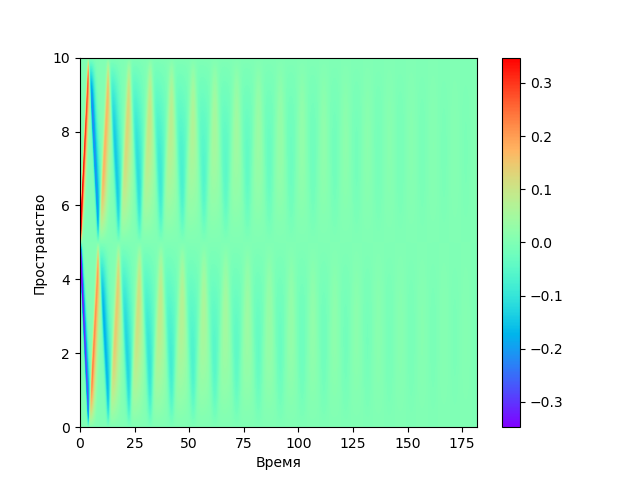
\includegraphics[height=0.4\textheight]{pics/task2/u-2-2-11_1.png}
    \caption{Проекция скорости для $\tau = 0.01, h = 0.01, \mu = 0.1, p(\rho) = \rho$}
\end{figure}

\begin{figure}[H]
    \centering
    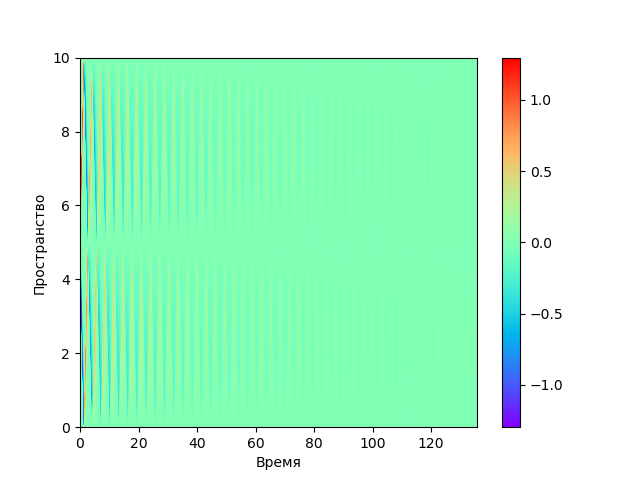
\includegraphics[height=0.4\textheight]{pics/task2/u-2-2-12_1.png}
    \caption{Проекция скорости для $\tau = 0.01, h = 0.01, \mu = 0.1, p(\rho) = 10\rho$}
\end{figure}

\begin{figure}[H]
    \centering
    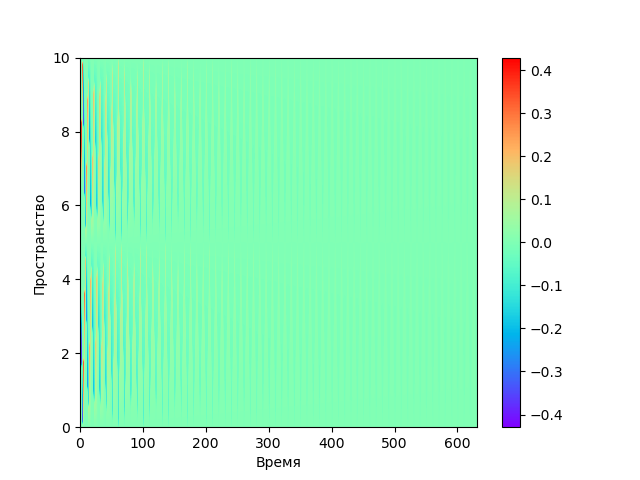
\includegraphics[height=0.4\textheight]{pics/task2/u-2-2-21_1.png}
    \caption{Проекция скорости для $\tau = 0.01, h = 0.01, \mu = 0.01, p(\rho) = \rho$}
\end{figure}

\begin{figure}[H]
    \centering
    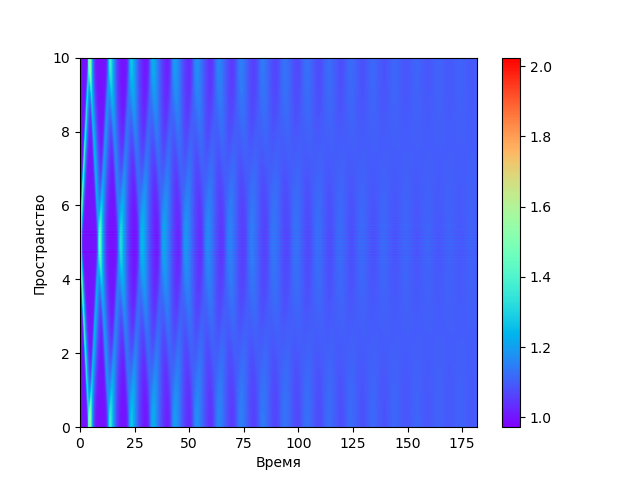
\includegraphics[height=0.4\textheight]{pics/task2/h-2-2-11_1.png}
    \caption{Проекция плотности для $\tau = 0.01, h = 0.01, \mu = 0.1, p(\rho) = \rho$}
\end{figure}

\begin{figure}[H]
    \centering
    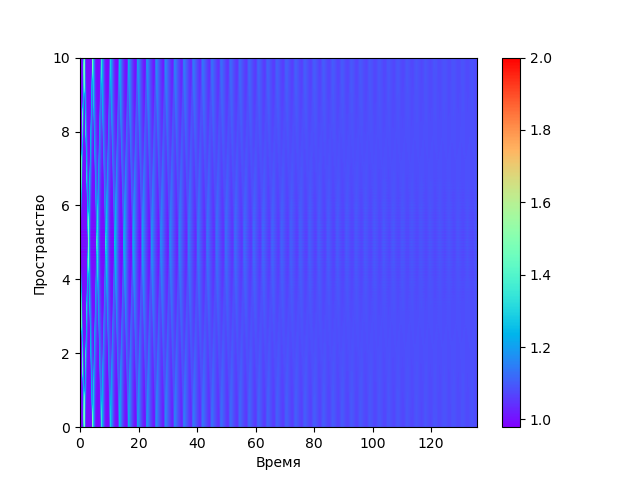
\includegraphics[height=0.4\textheight]{pics/task2/h-2-2-12_1.png}
    \caption{Проекция плотности для $\tau = 0.01, h = 0.01, \mu = 0.1, p(\rho) = 10\rho$}
\end{figure}

\begin{figure}[H]
    \centering
    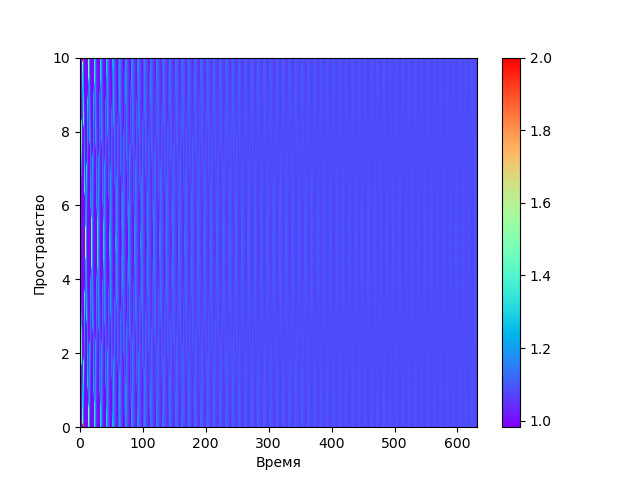
\includegraphics[height=0.4\textheight]{pics/task2/h-2-2-21_1.png}
    \caption{Проекция плотности для $\tau = 0.01, h = 0.01, \mu = 0.01, p(\rho) = \rho$}
\end{figure}
\end{center}

На графиках с одинаковой зависимостью $p$ от $\rho$ видно, что длина цикла примерно одинакова и лежит между 9 и 10, но при этом при меньшей вязкости стабилизация происходит медленнее. При большем коэффициенте зависимости длина цикла уменьшилась.

\begin{figure}[h]
	\begin{minipage}[h]{0.47\linewidth}
		\centering
		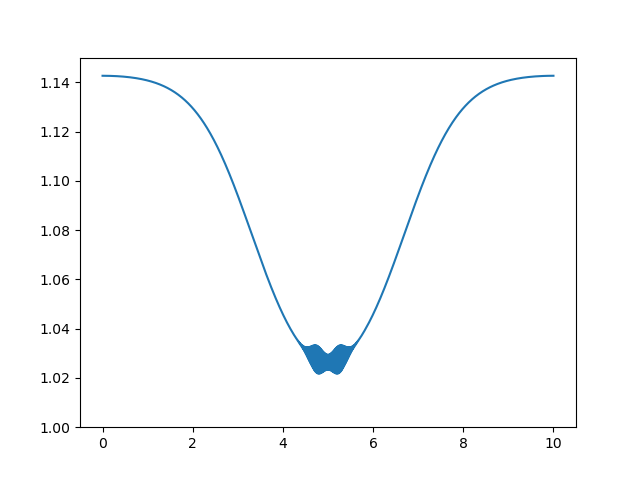
\includegraphics[width=1\linewidth]{pics/task2/14h_1.png} 
		\caption{Плотность на слое $n_{st} / 4$}
	\end{minipage}
	\hfill
	\begin{minipage}[h]{0.47\linewidth}
		\centering
		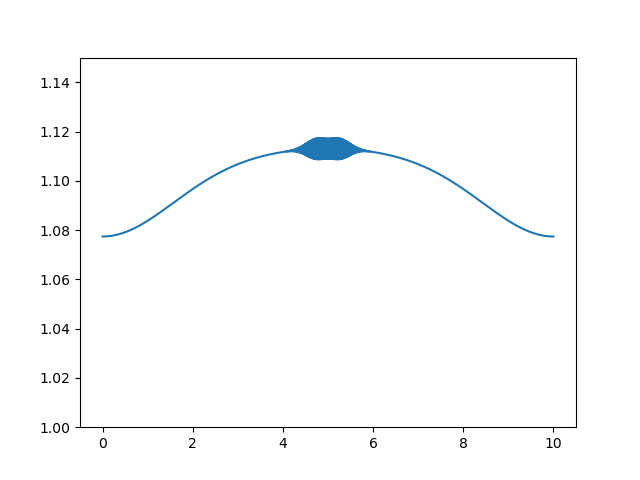
\includegraphics[width=1\linewidth]{pics/task2/24h_1.png} 
		\caption{Плотность на слое $n_{st} / 2$}
	\end{minipage}
	\vfill
	\begin{minipage}[h]{0.47\linewidth}
		\centering
		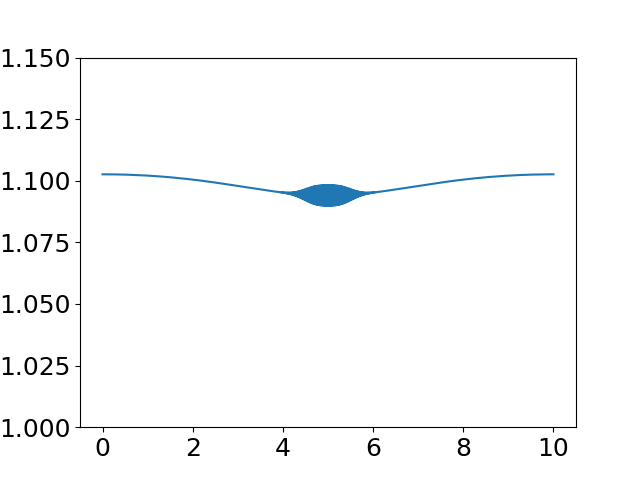
\includegraphics[width=1\linewidth]{pics/task2/34h_1.png} 
		\caption{Плотность на слое $3n_{st} / 4$}
	\end{minipage}
	\hfill
	\begin{minipage}[h]{0.47\linewidth}
		\centering
		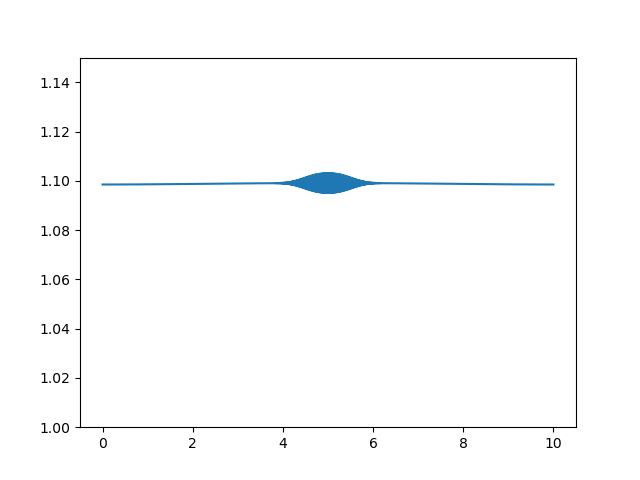
\includegraphics[width=1\linewidth]{pics/task2/44h_1.png} 
		\caption{Плотность на слое $n_{st}$}
	\end{minipage}
	\caption{Графики плотности для $\tau = 0.01, h = 0.01, \mu = 0.1, p(\rho) = \rho$}
\end{figure}

\begin{figure}[h]
	\begin{minipage}[h]{0.47\linewidth}
		\centering
		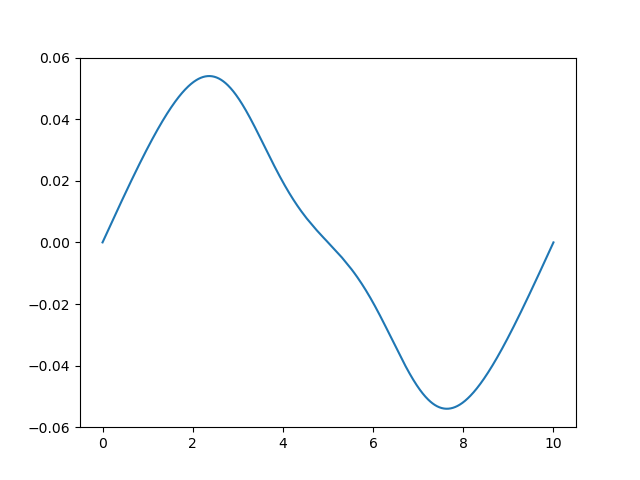
\includegraphics[width=1\linewidth]{pics/task2/14u_1.png} 
		\caption{Скорость на слое $n_{st} / 4$}
	\end{minipage}
	\hfill
	\begin{minipage}[h]{0.47\linewidth}
		\centering
		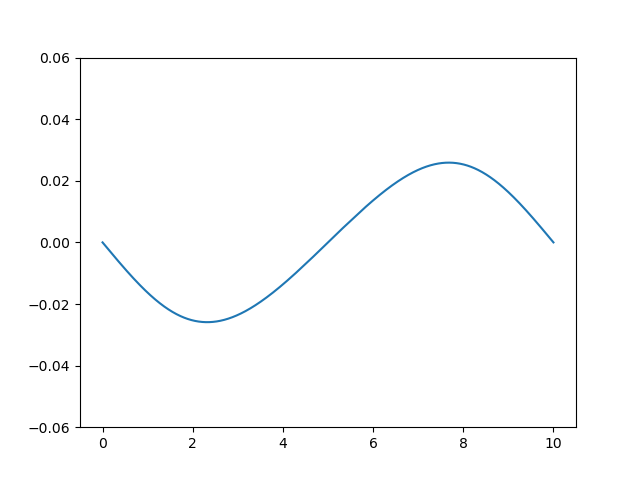
\includegraphics[width=1\linewidth]{pics/task2/24u_1.png} 
		\caption{Скорость на слое $n_{st} / 2$}
	\end{minipage}
	\vfill
	\begin{minipage}[h]{0.47\linewidth}
		\centering
		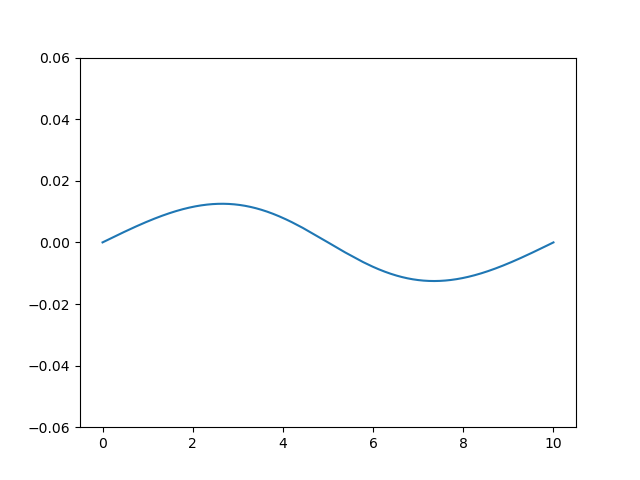
\includegraphics[width=1\linewidth]{pics/task2/34u_1.png} 
		\caption{Скорость на слое $3n_{st} / 4$}
	\end{minipage}
	\hfill
	\begin{minipage}[h]{0.47\linewidth}
		\centering
		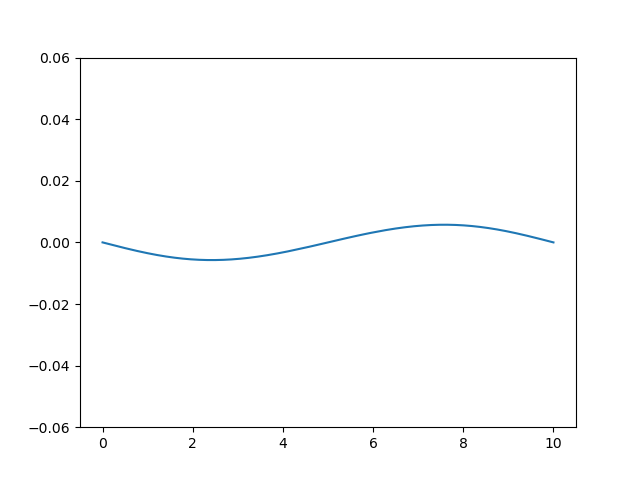
\includegraphics[width=1\linewidth]{pics/task2/44u_1.png} 
		\caption{Скорость на слое $n_{st}$}
	\end{minipage}
	\caption{Графики скорости для $\tau = 0.01, h = 0.01, \mu = 0.1, p(\rho) = \rho$}
\end{figure}

\begin{tabular}{*{6}{|l}|}
    \hline
    \multicolumn{6}{|c|}{$\mu = 0.001, p(\rho) = 1\rho, h = , \tau = $} \\
    \hline
    &$n_{st}/4 $&$ n_{st}/2$&$3n_{st}/4$&$n_{st}$&$T_{st}$ \\
    \hline
\end{tabular}

\begin{tabular}{*{6}{|l}|}
    \hline
    \multicolumn{6}{|c|}{$\mu = 0.001, p(\rho) = 1\rho, h = , \tau = $} \\
    \hline
    &$n_{st}/4 $&$ n_{st}/2$&$3n_{st}/4$&$n_{st}$&$T_{st}$ \\
    \hline
\end{tabular}

\begin{tabular}{*{6}{|l}|}
    \hline
    \multicolumn{6}{|c|}{$\mu = 0.001, p(\rho) = 1\rho, h = , \tau = $} \\
    \hline
    &$n_{st}/4 $&$ n_{st}/2$&$3n_{st}/4$&$n_{st}$&$T_{st}$ \\
    \hline
\end{tabular}

\begin{tabular}{*{6}{|l}|}
    \hline
    \multicolumn{6}{|c|}{$\mu = 0.001, p(\rho) = 1\rho, h = , \tau = $} \\
    \hline
    &$n_{st}/4 $&$ n_{st}/2$&$3n_{st}/4$&$n_{st}$&$T_{st}$ \\
    \hline
\end{tabular}

\begin{tabular}{*{6}{|l}|}
    \hline
    \multicolumn{6}{|c|}{$\mu = 0.001, p(\rho) = 1\rho, h = , \tau = $} \\
    \hline
    &$n_{st}/4 $&$ n_{st}/2$&$3n_{st}/4$&$n_{st}$&$T_{st}$ \\
    \hline
\end{tabular}

\begin{tabular}{*{6}{|l}|}
    \hline
    \multicolumn{6}{|c|}{$\mu = 0.001, p(\rho) = 1\rho, h = , \tau = $} \\
    \hline
    &$n_{st}/4 $&$ n_{st}/2$&$3n_{st}/4$&$n_{st}$&$T_{st}$ \\
    \hline
\end{tabular}

\begin{tabular}{*{6}{|l}|}
    \hline
    \multicolumn{6}{|c|}{$\mu = 0.001, p(\rho) = 1\rho, h = , \tau = $} \\
    \hline
    &$n_{st}/4 $&$ n_{st}/2$&$3n_{st}/4$&$n_{st}$&$T_{st}$ \\
    \hline
\end{tabular}



\end{document}
